\section{Pedagogical Design}
\label{sec:pedagogy}

Each design choice described in Sections~\ref{sec:architecture}
and~\ref{sec:circuit-solver} was made with a specific misconception or missing intuition in
mind, in the spirit of Papert's constructionism~\cite{papert1980mindstorms}: a learner
constructs a working artifact and inspects its behavior directly, rather than observing that
behavior secondhand.

\textbf{Wiring as physical placement, not schematic capture.} A component's two leads are
specific block faces, and two blocks are electrically connected only if each presents a
conductive face to the other. This arrangement is closer to breadboarding than to drawing a
schematic: a player who wires a resistor and a capacitor in what is intended to be a series
loop, but leaves a gap, obtains a demonstrably incomplete circuit (Section~\ref{sec:circuit-solver}'s
floating-node handling ensures this fails safely rather than crashing), in the same way that
a breadboard with a missing jumper simply does not function, rather than a schematic tool
flagging an unconnected pin as an abstract error.

\textbf{An explicit ground reference.} The observation that voltage is always relative to a
chosen reference is a standard remark in an introductory course, but a student may easily
receive it as incidental rather than consequential, because a schematic tool typically draws
a ground symbol automatically, already connected, wherever an exercise requires one.
Requiring a player to place a ground block and wire it in independently, before a wire's
absolute voltage reading becomes meaningful (Section~\ref{sec:circuit-solver}), renders the
reference an object for which the player is responsible, rather than a background
assumption.

\textbf{Sources that must be switched on.} All three voltage sources -- power supply,
function generator, and AC Source -- are wired to a redstone input and remain inert until
that input is active: the first two an open circuit, contributing nothing to the solved
transient system; the AC Source a silenced 0~V excitation, contributing nothing to a Bode
sweep, since it never participates in the transient system at all
(Section~\ref{sec:ac-analysis}). This arrangement mirrors an actual laboratory
workflow (wire the circuit completely, verify it, and only then switch the bench supply on)
rather than a schematic tool's power sources, which are implicitly ``live'' the instant they
are drawn. It further allows a player to make, and recover from, the same wiring error a
bench technician must learn to avoid: an ideal voltage source whose two leads both terminate
at the same node is shorted across itself, regardless of whether the circuit exists inside a
game or in physical hardware, and the solver's defensive handling of this case
(Section~\ref{sec:circuit-solver}) ensures the error surfaces as an in-game warning to be
corrected, rather than as a crash.

\textbf{An oscilloscope capable of observing more than one signal at once.} A single-channel
readout answers the question of what a given component is doing in isolation, but the more
instructive classroom question is typically comparative: how does a capacitor's voltage lag
the source driving it, or how does a resistor's voltage track a memristor's drifting
resistance? Answering such questions requires observing multiple points simultaneously and
comparing their relative phase and shape, rather than only their instantaneous values in
isolation. Figure~\ref{fig:scope} shows the in-game oscilloscope pinned to three points
within the same circuit at once (a function generator, a capacitor, and a resistor),
reproducing the relative-phase comparison for which a bench oscilloscope's multiple channels
are ordinarily used.

\begin{figure*}[!t]
\centering
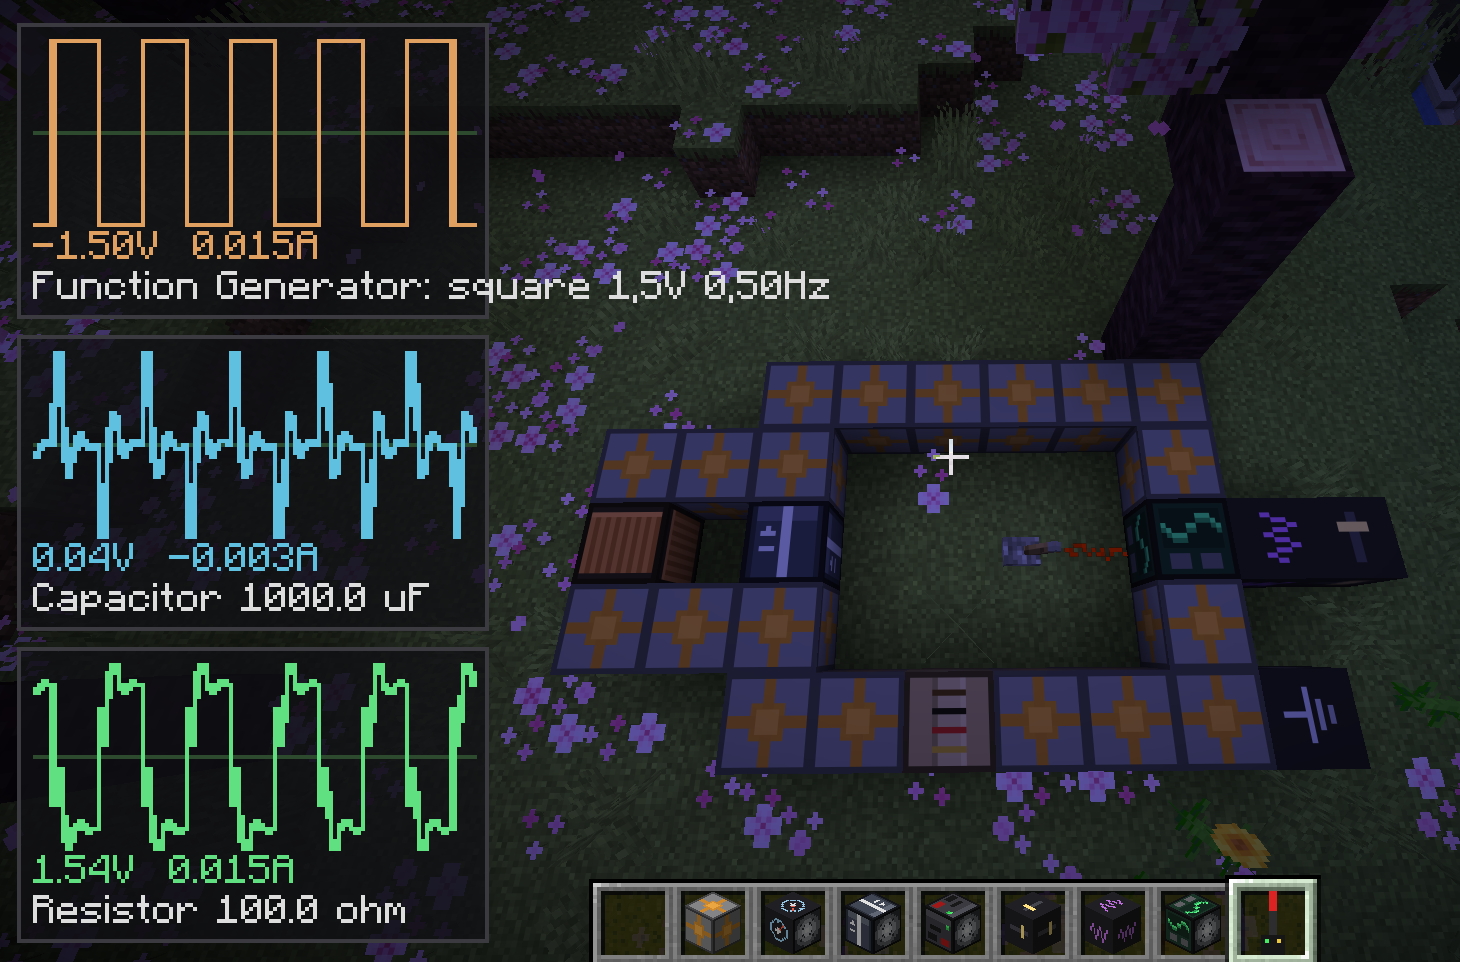
\includegraphics[width=0.48\textwidth]{figures/square_waveform.png}
\hfill
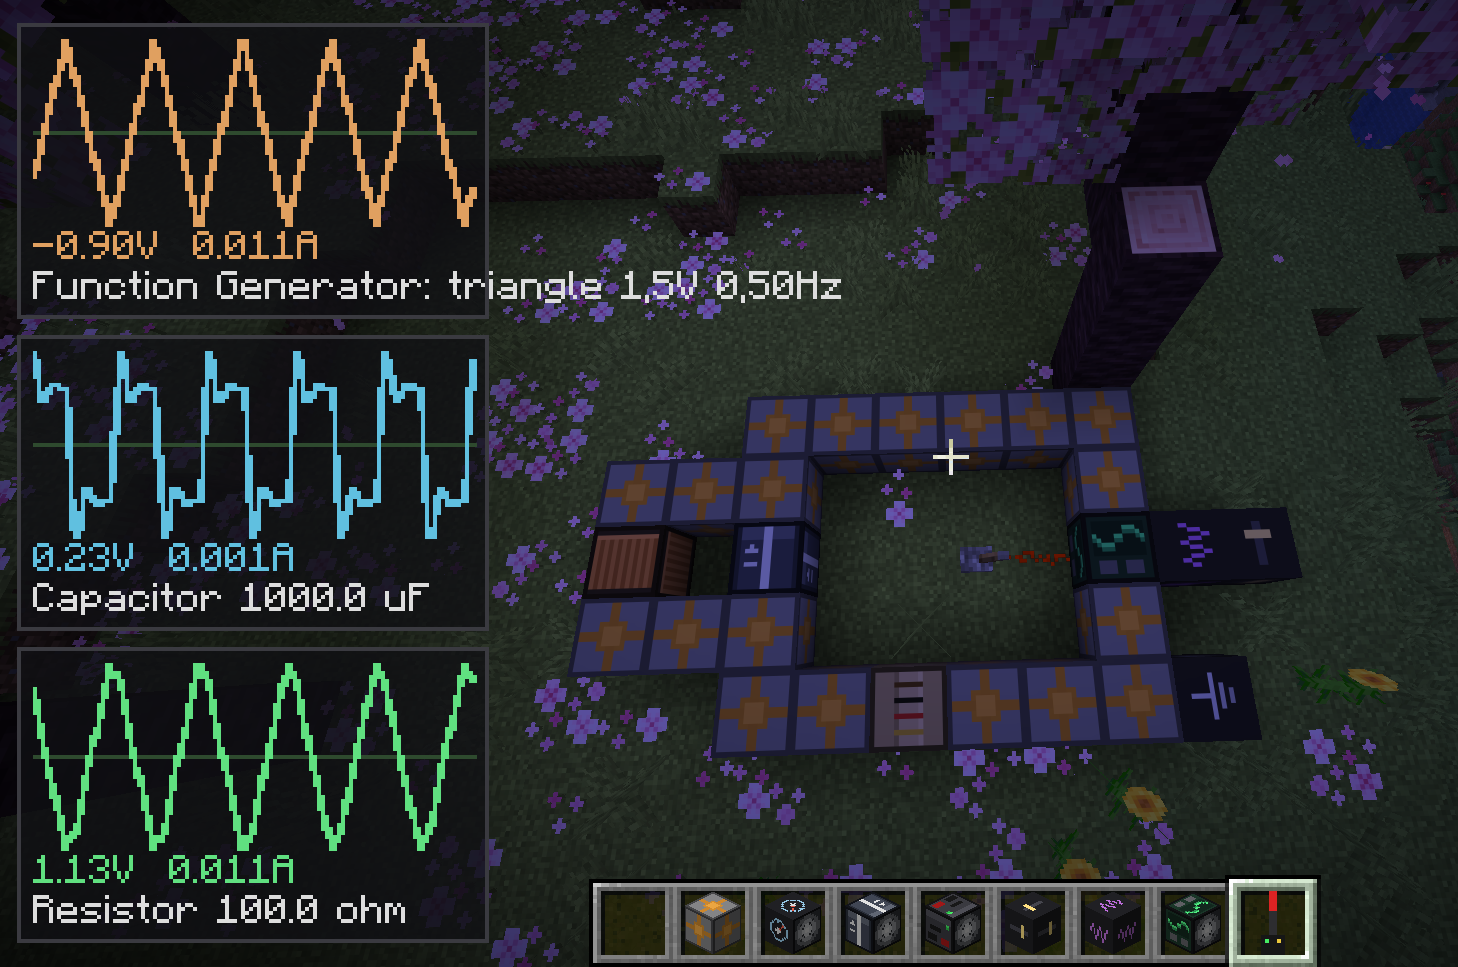
\includegraphics[width=0.48\textwidth]{figures/triangle_waveform.png}
\caption{The in-game multi-channel oscilloscope, pinned simultaneously to a function
generator (top trace), a capacitor (middle trace), and a resistor (bottom trace) within the
same circuit, driven by a square wave (left) and a triangle wave (right). Each trace is
independently auto-scaled and color-coded, with a live voltage/current readout and a summary
of that component's current state displayed below its plot.}
\label{fig:scope}
\end{figure*}
